
\chapter{Q-Learning}
待重读的资源:
\begin{itemize}
%\setlength{\itemsep}{0pt}
%\setlength{\parsep}{0pt}
\setlength{\parskip}{0pt}
\item[-]
\url{https://blog.csdn.net/qq_30615903/article/details/80739243}

\item[-]
\url{https://valohai.com/blog/reinforcement-learning-tutorial-part-1-q-learning/}

\item[-]
\url{https://www.baeldung.com/cs/epsilon-greedy-q-learning}
\end{itemize}

% https://blog.csdn.net/qq_30615903/article/details/80739243
% https://www.freecodecamp.org/news/an-introduction-to-q-learning-reinforcement-learning-14ac0b4493cc/

% 视频 https://v.youku.com/v_show/id_XMTk2NzM1Mjk5Mg==.html

% 发现了很多RL资料搬砖过来,刚入门的可以用得上

% David Silver 博士的 UCL 公开课:http://www0.cs.ucl.ac.uk/staff/d.silver/web/Teaching.html
% DeepMind 和 UCL 的DL、RL课程:https://www.youtube.com/playlist?list=PLqYmG7hTraZDNJre23vqCGIVpfZ_K2RZs
% Sergey Levine 的DRL课程:http://rail.eecs.berkeley.edu/deeprlcourse/
% OpenAI 的 Spinning Up in Deep RL:https://blog.openai.com/spinning-up-in-deep-rl/
% 关于深度强化学习良心paper:https://arxiv.org/abs/1810.06339

In reinforcement learning, the state-value function is usually denoted by $v$, 
while the action-value function is denoted by $q$.
The $q$ in $q$-learning is in fact refer to the action-value function. 
$Q$-learning is at the heart of all reinforcement learning algorithms.

%%%%%%%%%%%%%%%%%%%%%%%%%%%%%%%%%%%%%%%%%%%%%%%%%%%%%%%%
%
\section{What is $Q$-Learning ?}
%
%-------------------------------------------------------

$Q$-Learning is a Reinforcement learning policy that will find the next best action, 
given a current state. It chooses this action at random and aims to maximize the reward.

\begin{figure}[h]
\centering
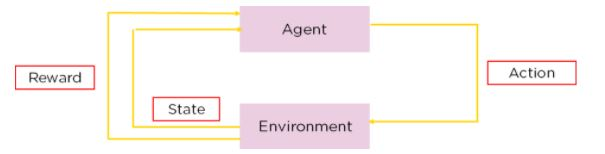
\includegraphics[scale=0.618]{pix/q_learning/3-components-q.jpg}
\caption{Components of Q-Learning}
%\label{fig:label}
\end{figure}

$Q$-learning is a model-free, off-policy reinforcement learning that will find the best 
course of action, given the current state of the agent. Depending on where the agent is 
in the environment, it will decide the next action to be taken.

Model-free means that the agent uses predictions of the environment's expected response 
to move forward. It does not use the reward system to learn, but rather, trial and error.

An example of $Q$-learning is an Advertisement recommendation system. In a normal ad 
recommendation system, the ads you get are based on your previous purchases or websites 
you may have visited. If you've bought a TV, you will get recommended TVs of different 
brands. 

\begin{figure}[h]
\centering

\includegraphics[scale=0.618]{pix/q_learning/4-adrecommend.jpg}
\caption{Ad Recommendation System}
%\label{fig:label}
\end{figure}

Using $Q$-learning, we can optimize the ad recommendation system to recommend products 
that are frequently bought together. The reward will be if the user clicks on the 
suggested product.

\begin{figure}[h]
\centering

\includegraphics[scale=0.618]{pix/q_learning/5-ad-q.jpg}
\caption{Ad Recommendation System with Q-Learning}
%\label{fig:label}
\end{figure}


\subsection{Important Terms in Q-Learning}

\begin{itemize}
%\setlength{\itemsep}{0pt}
%\setlength{\parsep}{0pt}
\setlength{\parskip}{0pt}
\item[1.]
States: The State, $S$, represents the current position of an agent in an environment.
\item[2.]
Action: The Action, $A$, is the step taken by the agent when it is in a particular state.
\item[3.]
Rewards: For every action, the agent will get a positive or negative reward.
\item[4.]
Episodes: When an agent ends up in a terminating state and can't take a new action.
\item[5.]
$Q$-Values: Used to determine how good an Action, $A$, taken at a particular state, $S$, 
is. $Q (A, S)$.
\item[6.]
Temporal Difference: A formula used to find the $Q$-Value by using the value of current 
state and action and previous state and action.
\end{itemize}


\subsection{What Is The Bellman Equation?}

The Bellman Equation is used to determine the value of a particular state and deduce 
how good it is to be in/take that state. The optimal state will give us the highest 
optimal value. 

The equation is given below. It uses the current state, and the reward associated with 
that state, along with the maximum expected reward and a discount rate, which determines 
its importance to the current state, to find the next state of our agent. The learning 
rate determines how fast or slow, the model will be learning. 

\begin{figure}[h]
\centering
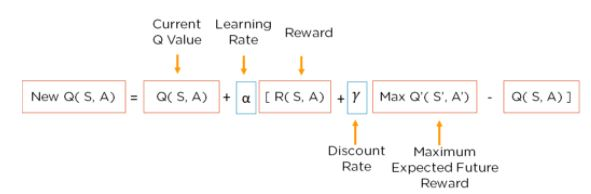
\includegraphics[scale=0.618]{pix/q_learning/6-bellman.jpg}
\caption{Bellman Equation}
%\label{fig:label}
\end{figure}


\subsection{A simplistic example}

Let's say that a robot has to cross a maze and reach the end point. There are mines, 
and the robot can only move one tile at a time. If the robot steps onto a mine, the 
robot is dead. The robot has to reach the end point in the shortest time possible.

The scoring/reward system is as below:
\begin{itemize}
%\setlength{\itemsep}{0pt}
%\setlength{\parsep}{0pt}
\setlength{\parskip}{0pt}
\item[1.]
The robot loses 1 point at each step. This is done so that the robot takes the 
shortest path and reaches the goal as fast as possible.

\item[2.]
If the robot steps on a mine, the point loss is 100 and the game ends.

\item[3.]
If the robot gets power \textcolor{magenta}{⚡️}, it gains 1 point.

\item[4.]
If the robot reaches the end goal, the robot gets 100 points.
\end{itemize}

Now, the obvious question is: {\bf How do we train a robot to reach the end goal 
with the shortest path without stepping on a mine?}

\begin{figure}[h]
\centering
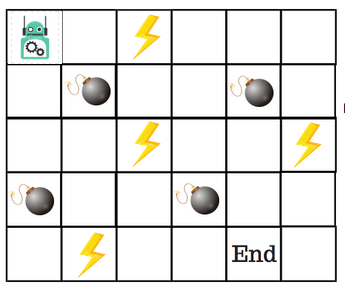
\includegraphics[scale=0.618]{pix/q_learning/q_robot_maze.png}
\caption{Maze}
%\label{fig:label}
\end{figure}
So, how do we solve this?


\subsection{Introducing the $Q$-Table}

\begin{tabular}{|c||c|c|}
\hline
$Q$-Table	& $a_1$	& $a_2$ \\
\hline
$s_1$	& $q(s_1,a_1)$	& $q(s_1,a_2)$ \\
\hline
$s_2$	& $q(s_2,a_1)$	& $q(s_2,a_2)$ \\
\hline
$s_3$	& $q(s_3,a_1)$	& $q(s_3,a_2)$ \\
\hline
\end{tabular}\;

\vspace

$Q$-Table is just a fancy name for a simple lookup table where we calculate the 
maximum expected future rewards for action at each state. Basically, this table 
will guide us to the best action at each state.

\begin{figure}[h]
\centering
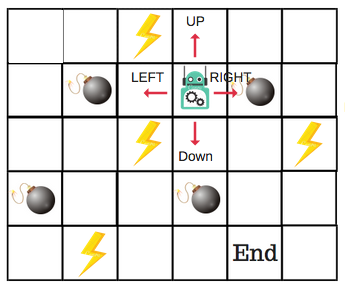
\includegraphics[scale=0.618]{pix/q_learning/q_robot_maze_actions.png}
\caption{Maze: actions}
%\label{fig:label}
\end{figure}
There will be four numbers of actions at each non-edge tile. When a robot is at a 
state it can either move up or down or right or left.

So, let's model this environment in our $Q$-Table.

In the $Q$-Table, the columns are the actions and the rows are the states.

\begin{figure}[h]
\centering
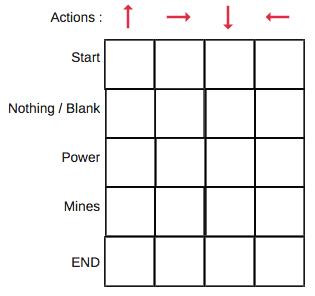
\includegraphics[scale=0.618]{pix/q_learning/q_robot_maze_table.png}
\caption{Maze: $q$-table}
%\label{fig:label}
\end{figure}

Each $Q$-table score will be the maximum expected future reward that the robot will 
get if it takes that action at that state. This is an iterative process, as we need 
to improve the $Q$-Table at each iteration.

But the questions are:

\begin{itemize}
%\setlength{\itemsep}{0pt}
%\setlength{\parsep}{0pt}
\setlength{\parskip}{0pt}
\item[-]
How do we calculate the values of the $Q$-table?
\item[-]
Are the values available or predefined?
\end{itemize}

To learn each value of the $Q$-table, we use the $Q$-Learning algorithm.


\subsection{How to Make a $Q$-Table?}

While running our algorithm, we will come across various solutions and the agent 
will take multiple paths. How do we find out the best among them? This is done by 
tabulating our findings in a table called a $Q$-Table.

A $Q$-Table helps us to find the best action for each state in the environment. We 
use the Bellman Equation at each state to get the expected future state and reward 
and save it in a table to compare with other states. 

Lets us create a $q$-table for an agent that has to learn to run, fetch and sit on 
command. The steps taken to construct a $q$-table are :

{\bf Step 1}: Create an initial $Q$-Table with all values initialized to $0$

When we initially start, the values of all states and rewards will be $0$. Consider 
the $Q$-Table shown below which shows a dog simulator learning to perform actions :

\begin{figure}[h]
\centering
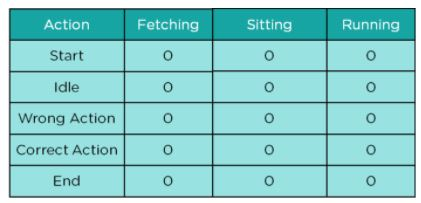
\includegraphics[scale=0.618]{pix/q_learning/7-initial.jpg}
\caption{Initial $q$-table}
%\label{fig:label}
\end{figure}

{\bf Step 2}: Choose an action and perform it. Update values in the $q$-table

This is the starting point. We have performed no other action as of yet. Let us say 
that we want the agent to sit initially, which it does. The table will change to:

\begin{figure}[h]
\centering
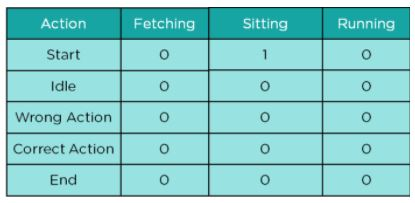
\includegraphics[scale=0.618]{pix/q_learning/8-qtable.jpg}
\caption{$Q$-table after performing an action}
%\label{fig:label}
\end{figure}

{\bf Step 3}: Get the value of the reward and calculate the value $Q$-Value using 
Bellman Equation

For the action performed, we need to calculate the value of the actual reward and 
the $Q( S, A )$ value

\begin{figure}[h]
\centering
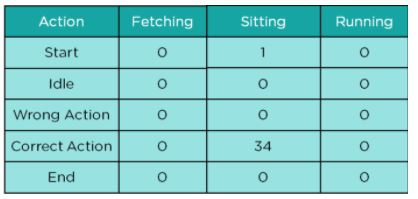
\includegraphics[scale=0.618]{pix/q_learning/9-updatingq.jpg}
\caption{Updating $q$-table with Bellman Equation}
%\label{fig:label}
\end{figure}

{\bf Step 4}: Continue the same until the table is filled or an episode ends

The agent continues taking actions and for each action, the reward and $Q$-value are 
calculated and it updates the table.

\begin{figure}[h]
\centering
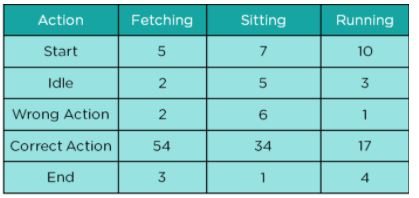
\includegraphics[scale=0.618]{pix/q_learning/10-finalq.jpg}
\caption{Final $q$-table at end of an episode}
%\label{fig:label}
\end{figure}


%%%%%%%%%%%%%%%%%%%%%%%%%%%%%%%%%%%%%%%%%%%%%%%%%%%%%%%%
%
\section{Mathematics behind the Q-Learning algorithm}
%
%-------------------------------------------------------

\subsection{Q-function}

The Q-function uses the Bellman equation and takes two inputs: state (s) and action (a).

\begin{figure}[h]
\centering
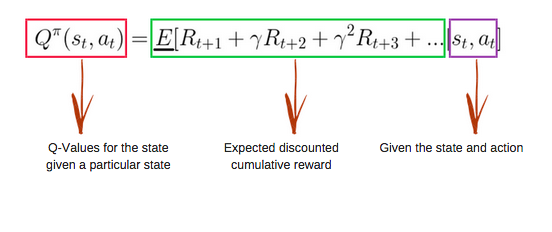
\includegraphics[scale=0.618]{pix/q_learning/q_function.png}
\caption{Maze: q-function}
%\label{fig:label}
\end{figure}

Using the above function, we get the values of Q for the cells in the table.

When we start, all the values in the Q-table are zeros.

There is an iterative process of updating the values. As we start to explore the 
environment, the Q-function gives us better and better approximations by continuously 
updating the Q-values in the table.

Now, let's understand how the updating takes place.


\subsection{Introducing the $Q$-learning algorithm process}

\begin{figure}[h]
\centering
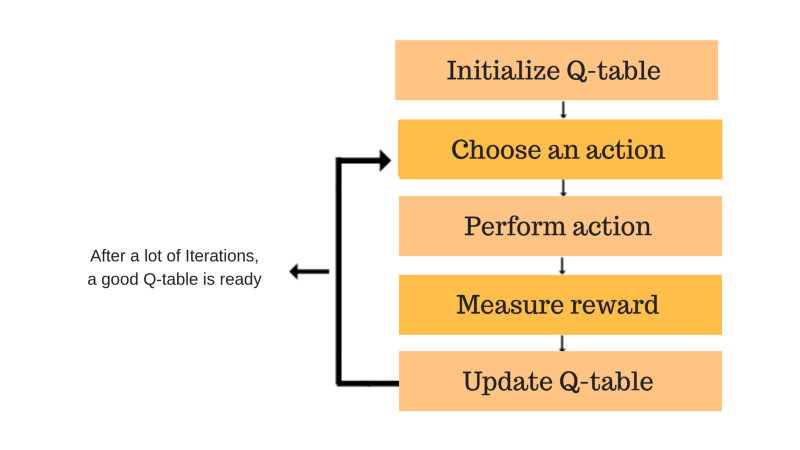
\includegraphics[scale=0.4]{pix/q_learning/q_learning_algorithm_process.png}
\caption{Maze: algorithm process}
%\label{fig:label}
\end{figure}
Each of the colored boxes is one step. Let's understand each of these steps in detail.


\subsubsection{Step 1: initialize the $Q$-Table}
We will first build a $Q$-table. There are $n$ columns, where $n=$ number of actions. 
There are m rows, where m= number of states. We will initialise the values at 0.

\begin{figure}[h]
\centering
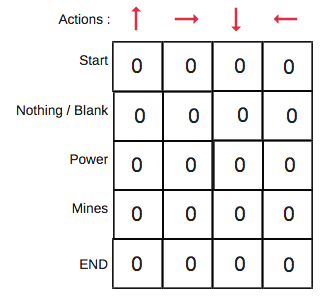
\includegraphics[scale=0.5]{pix/q_learning/q_robot_maze_table_init.png}
\caption{Maze: q-table initialization}
%\label{fig:label}
\end{figure}
In our robot example, we have four actions ($a=4$) and five states ($s=5$). So we will 
build a table with four columns and five rows.


\subsubsection{Steps 2 and 3: choose and perform an action}

This combination of steps is done for an undefined amount of time. This means that 
this step runs until the time we stop the training, or the training loop stops as 
defined in the code.

We will choose an action ($a$) in the state ($s$) based on the $Q$-Table. But, as 
mentioned earlier, when the episode initially starts, every $Q$-value is $0$.

So now the concept of exploration and exploitation trade-off comes into play. This 
chapter has more details.

We'll use something called the {\bf epsilon greedy strategy}.

In the beginning, the epsilon rates will be higher. The robot will explore the 
environment and randomly choose actions. The logic behind this is that the robot 
does not know anything about the environment.

As the robot explores the environment, the epsilon rate decreases and the robot 
starts to exploit the environment.

During the process of exploration, the robot progressively becomes more confident in 
estimating the $Q$-values.

For the robot example, there are four actions to choose from: up, down, left, and 
right. We are starting the training now — our robot knows nothing about the 
environment. So the robot chooses a random action, say right.

\begin{figure}[h]
\centering
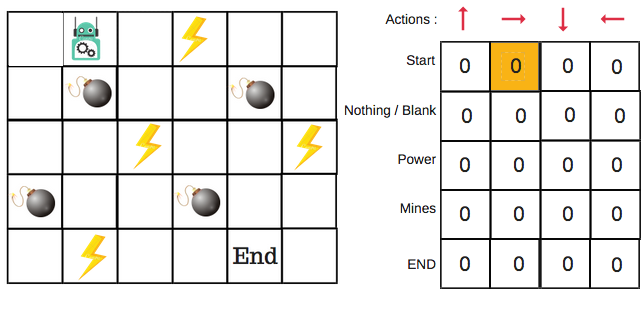
\includegraphics[scale=0.5]{pix/q_learning/q_robot_maze_perform_action.png}
\caption{Maze: perform an action}
%\label{fig:label}
\end{figure}

We can now update the $Q$-values for being at the start and moving right using the 
Bellman equation.


\subsubsection{Steps 4 and 5: evaluate}

Now we have taken an action and observed an outcome and reward. We need to update 
the function $Q(s,a)$.

\begin{figure}[h]
\centering
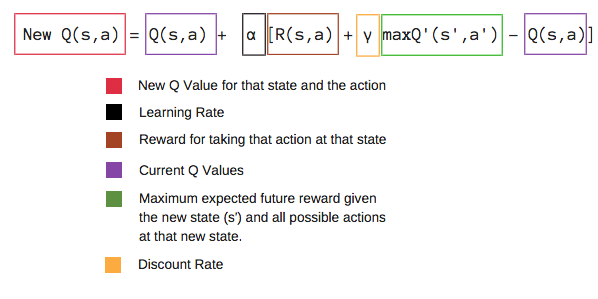
\includegraphics[scale=0.5]{pix/q_learning/q_robot_maze_q_function.png}
\caption{Maze: q-function}
%\label{fig:label}
\end{figure}

In the case of the robot game, to reiterate the scoring/reward structure is:

\begin{itemize}
%\setlength{\itemsep}{0pt}
%\setlength{\parsep}{0pt}
\setlength{\parskip}{0pt}
\item[-]
power $= +1$
\item[-]
mine $= -100$
\item[-]
end $= +100$
\end{itemize}

\begin{figure}[h]
\centering
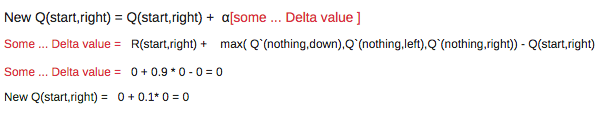
\includegraphics[scale=0.7]{pix/q_learning/q_robot_maze_iteration.png}
%\caption{Maze: q-function}
%\label{fig:label}
\end{figure}
We will repeat this again and again until the learning is stopped. In this way 
the $Q$-Table will be updated.


%%%%%%%%%%%%%%%%%%%%%%%%%%%%%%%%%%%%%%%%%%%%%%%%%%%%%%%%
%
\section{Implementation using python}
%
%-------------------------------------------------------

Let's use $Q$-Learning to find the shortest path between two points. We have a group 
of nodes and we want the model to automatically find the shortest way to travel from 
one node to another. We start by importing the necessary modules:

\begin{lstlisting}[language=Python]
import numpy as np
\end{lstlisting}

Then we define all possible actions or the points/nodes that exist.
\begin{lstlisting}[language=Python]
# Define the actions
actions = [0,1,2,3,4,5,6,7,8]
\end{lstlisting}

We define the rewards array for every action.
\begin{lstlisting}[language=Python]
# Define the rewards
rewards = np.array([[0,1,0,0,0,0,0,0,0],
[1,0,1,0,1,0,0,0,0],
[0,1,0,0,0,1,0,0,0],
[0,0,0,0,0,0,1,0,0],
[0,1,0,0,0,0,0,1,0],
[0,0,1,0,0,0,0,0,0],
[0,0,0,1,0,0,0,1,0],
[0,0,0,0,1,0,1,0,1],
[0,0,0,0,0,0,0,1,0]])
\end{lstlisting}

% https://www.simplilearn.com/tutorials/machine-learning-tutorial/what-is-q-learning


\subsection{公式推导}

% https://blog.csdn.net/qq_30615903/article/details/80739243

举个例子如图有一个 GridWorld 的游戏从起点出发到达终点为胜利掉进陷阱为失败。智能体(Agent)、
环境状态(environment)、奖励(reward)、动作(action)可以将问题抽象成一个马尔科夫决策过程,
我们在每个格子都算是一个状态 $s_t$, $\pi(a|s)$ 在 $s$ 状态下采取动作 $a$ 策略 。 
$P(s'|s,a)$ 也可以写成 $P_{ss'}^a$ 为在 $s$ 状态下选择 $a$ 动作转换到下一个状态 $s'$ 的概率。
$R(s'|s,a)$ 表示在 $s$ 状态下采取 $a$ 动作转移到 $s'$ 的奖励 reward,
我们的目的很明确就是找到一条能够到达终点获得最大奖赏的策略。

An agent is in the bottom left cell of a grid. The grey cell is a wall. The two coloured 
cells give a reward. There is a reward of $1$ of being in the top-right (diamond) cell, 
but a negative value of $-1$ for the cell immediately below (explosive).

\begin{figure}[h]
\centering
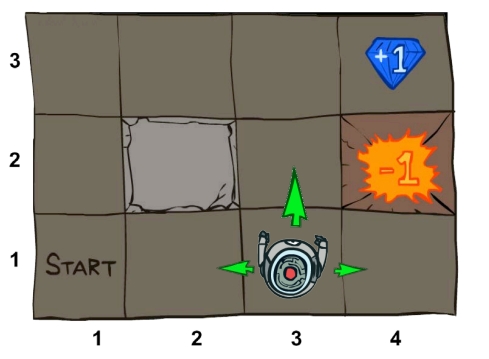
\includegraphics[scale=0.7]{pix/q_learning/gridworld.png}
%\caption{Example: Gridworld}
%\label{fig:label}
\end{figure}

问题模型 -- An MDP defined by:
\begin{itemize}
%\setlength{\itemsep}{0pt}
%\setlength{\parsep}{0pt}
\setlength{\parskip}{0pt}
\item[-]
Set of states $\mathcal{S}$

\item[-]
Set of actions $\mathcal{A}$

\item[-]
Transition function $P(s'|s, a)$

\item[-]
Reward function $R(s,a,s')$

\item[-]
Start state $s_0$

\item[-]
Discount factor $\gamma$

\item[-]
Horizon $H$

\end{itemize}


目标:找到使得累计奖励期望值最大的策略
$$
\max_\pi E\left[ \sum_{t=0}^H \gamma^t R(S_t, A_t, S_{t+1}) | \pi \right]
$$

$Q$-learning 的主要优势就是使用了时间差分法TD(融合了蒙特卡洛和动态规划)能够进行离线学习, 
使用 Bellman 方程可以对马尔科夫过程求解最优策略。


%%%%%%%%%%%%%%%%%%%%%%%%%%%%%%%%%%%%%%%%%%%%%%%%%%%%%%%%
%
\section{Deep $Q$-Learning - Combining Neural Networks And RL}
%
%-------------------------------------------------------

% https://deeplizard.com/learn/video/wrBUkpiRvCA

In this section, we'll bring artificial neural networks into our discussion of RL. 
Specifically, we'll be building on the concept of $Q$-learning we've discussed over 
the last few sections to introduce the concept of deep $Q$-learning and deep $Q$-networks 
(or DQNs). This will move us into the world of deep reinforcement learning.

DQN 为了解决动作空间过大造成维数灾难问题在Q-learning的基础上引入了神经网络。DQN 主要是把 $Q$ 
函数通过价值函数近似方法转换为一个深度神经网络。神经网络输入的是状态,输出每个动作的 $Q$ 值。

前面介绍的 $Q$-learning 是一种 value-based 方法,不是学习策略,而是说有一个 critic 通过 
MC based 的方法或者 TD based 的方法得出状态值函数 $V_\pi(s)$ 进行 Policy Evaluation 
(策略评估)。


\subsection{Limitations Of $Q$-Learning With Value Iteration}

From everything we've discussed over the last few sections, we should now be comfortable 
with the idea of $Q$-learning. Now, while it's true that the $Q$-learning algorithm that 
we used to play games may do a pretty decent job in relatively small state spaces, it's 
performance will drop-off considerably when we work in more complex and sophisticated 
environments.

In \href{https://deeplizard.com/learn/video/QK_PP_2KgGE}{Frozen Lake}, for example, our 
environment was relatively simplistic with only 16 states and 4 actions, giving us a 
total state-action space of just 16 x 4. Meaning we only had 16 x 4 or 64 $Q$-values to 
update in the $Q$-table. Given the fact that these $Q$-value updates occur in an iterative 
fashion, we can imagine that as our state space increases in size, the time it will take 
to traverse all those states and iteratively update the $Q$-values will also increase.

Think about a video game where a player has a large environment to roam around in. Each 
state in the environment would be represented by a set of pixels, and the agent may be 
able to take several actions from each state. The iterative process of computing and 
updating $Q$-values for each state-action pair in a large state space becomes 
computationally inefficient and perhaps infeasible due to the computational resources 
and time this may take.

So, what can we do when we want to step up our game from a simple toy environment, like 
Frozen Lake, to something more sophisticated? Well, rather than using value iteration to 
directly compute $Q$-values and find the optimal $Q$-function, we instead use a function 
approximation to estimate the optimal $Q$-function.

Well, you know what can do a pretty darn good job at approximating functions? Artificial 
Neural Networks!


\subsection{Deep $Q$-Learning}

% https://pytorch.org/tutorials/intermediate/reinforcement_q_learning.html

We'll make use of a deep neural network to estimate the $Q$-values for each state-action 
pair in a given environment, and in turn, the network will approximate the optimal 
$Q$-function. The act of combining $Q$-learning with a deep neural network is called 
deep $Q$-learning, and a deep neural network that approximates a $Q$-function is called 
a deep $Q$-Network, or DQN.

\begin{equation}\label{eq:dqn_bellman_equation}
q_*(s,a) = E \left[ R_{t+1} + \gamma\max_{a'}q_*(s', a')
\right]
\end{equation}

\begin{emp_box}
$R_{t+1}$ 即所谓 immediate reward, 而 $\gamma\max_{a'}q_*(s', a')$ 为 future reward with 
discount rate $\gamma$。这里隐含存在最优 policy 使得达到 future reward 的最大化。

The main idea behind $Q$-learning is that if we had a function 
$q_*: State \times Action \rightarrow \mathbb{R}$, that could tell us what our return 
would be, if we were to take an action in a given state, then we could easily construct 
a policy that maximizes our rewards:
$$
\pi_*(s) = \arg\max_a q_*(s,a)
$$
\end{emp_box}

However, we don't know everything about the world, so we don't have access to $q_*$. 
But, since neural networks are universal function approximators, we can simply create 
one and train it to resemble $q_*$.

For our training update rule, we'll use a fact that every $Q$ function for some policy 
obeys the Bellman equation:
$$
q_\pi(s,a) = r + \gamma q_\pi(s', \pi(s'))
$$
\noindent{}The difference between the two sides of the equality is known as the temporal 
difference error:
$$
\delta = q(s,a) - (r + \gamma \max_a q(s', a))
$$
\noindent{}To minimise this error, we will use the Huber loss. The Huber loss acts like 
the mean squared error when the error is small, but like the mean absolute error when 
the error is large - this makes it more robust to outliers when the estimates of $Q$ 
are very noisy. We calculate this over a batch of transitions, $B$, sampled from the 
replay memory:
$$
\mathcal{L} = \frac{1}{|B|} \sum_{(s,a,s',r)\in B} \mathcal{L}(\delta)
$$
\noindent{}where
$$
\mathcal{L}(\delta) = \begin{cases}
\frac{1}{2}\delta^2 &\text{for} |\delta| \leq 1, \\
|\delta| - \frac{1}{2} &\text{otherwise.}
\end{cases}
$$

Let's break down how exactly this integration of neural networks and $Q$-learning works. 
We'll first discuss this at a high level, and then we'll get into all the nitty-gritty 
details.


\subsection{Deep $Q$-Networks}

Suppose we have some arbitrary deep neural network that accepts states from a given 
environment as input. For each given state input, the network outputs estimated $Q$-values 
for each action that can be taken from that state. The objective of this network is to 
approximate the optimal $Q$-function, and remember that the optimal $Q$-function will 
satisfy the Bellman equation that we covered previously:

With this in mind, the loss from the network is calculated by comparing the outputted 
$Q$-values to the target $Q$-values from the right hand side of the Bellman equation, 
and as with any network, the objective here is to minimize this loss.

\begin{figure}[h]
\centering
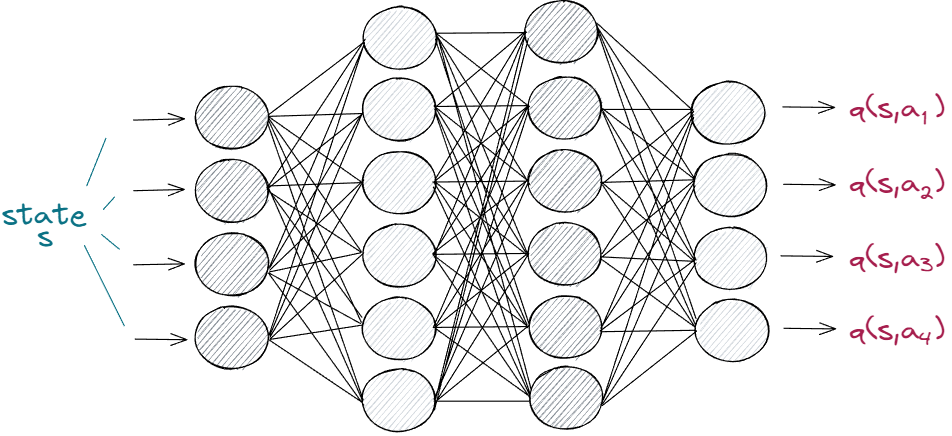
\includegraphics[scale=0.618]{pix/q_learning/q_network.png}
\caption{DQN states actions}
%\label{fig:label}
\end{figure}

After the loss is calculated, the weights within the network are updated via SGD and 
backpropagation, again, just like with any other typical network. This process is done 
over and over again for each state in the environment until we sufficiently minimize 
the loss and get an approximate optimal $Q$-function.

So, take a second now to think about how we previously used the Bellman equation to 
compute and update $Q$-values in our $Q$-table in order to find the optimal $Q$-function. 
Now, with deep $Q$-learning, our network will make use of the Bellman equation to estimate 
the $Q$-values to find the optimal $Q$-function. So, we're still solving the same general 
problem here, just with a different algorithm. Rather than making use of value iteration 
to solve the problem, we're now using a deep neural network.

Alright, we should now have a general idea about what deep $Q$-learning is and what, at 
a high level, the deep $Q$-network is doing. Now, let's get a little more into the details 
about the network itself.


\subsubsection{The Input}

We know that the network would accept states from the environment as input. Thinking of 
Grid world example, we could easily represent the states using a simple coordinate system 
from the grid of the environment and use this as input.

If we're in a more complex environment, though, like a video game, for example, then 
we'll use images as our input. Specifically, we'll use still frames that capture states 
from the environment as the input to the network.

The standard preprocessing done on the frames usually involves converting the RGB data 
into grayscale data since the color in the image is probably usually not going to affect 
the state of the environment. Additionally, we'll typically see some cropping and scaling 
as well to both cut out unimportant information from the frame and shrink the size of 
the image.

Now actually, rather than having a single frame represent a single input, we usually 
will use a stack of a few consecutive frames to represent a single input. So, we would 
grab, say, four consecutive frames from the video game. We'd then do all the preprocessing 
on each of these four frames we mentioned earlier – the grayscale conversion, the 
cropping, and the scaling – and then we'd take the preprocessed frames and stack them on 
top of each other in the order of which they occurred in the game.

\begin{figure}[h]
\centering
\begin{minipage}{0.49\linewidth}
  \centering
  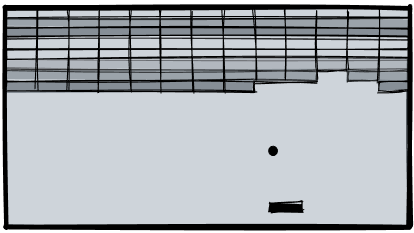
\includegraphics[width=0.618\linewidth]{pix/q_learning/game_1.png}
%  \caption{Gambler event.}
%  \label{fig:dp_gambler_event}
\end{minipage}%
\begin{minipage}{0.49\linewidth}
  \centering
  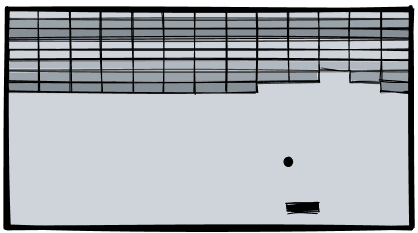
\includegraphics[width=0.618\linewidth]{pix/q_learning/game_2.png}
%  \caption{Gambler event list.}
%  \label{fig:dp_gambler_event_list}
\end{minipage}
\end{figure}

\begin{figure}[h]
\centering
\begin{minipage}{0.49\linewidth}
  \centering
  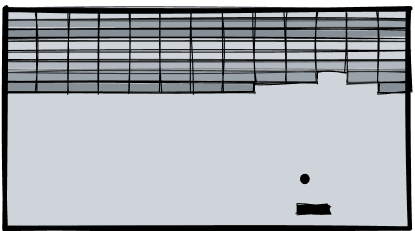
\includegraphics[width=0.618\linewidth]{pix/q_learning/game_3.png}
%  \caption{Gambler event.}
%  \label{fig:dp_gambler_event}
\end{minipage}%
\begin{minipage}{0.49\linewidth}
  \centering
  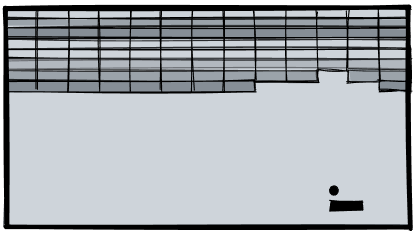
\includegraphics[width=0.618\linewidth]{pix/q_learning/game_4.png}
%  \caption{Gambler event list.}
%  \label{fig:dp_gambler_event_list}
\end{minipage}
\end{figure}

We do this because a single frame usually isn't going to be enough for our network, 
or even for our human brains, to fully understand the state of the environment. For 
example, by just looking at the first single frame above from the Atari game, 
Breakout, we can't tell if the ball is coming down to the paddle or going up to hit 
the block. We also don't have any indication about the speed of the ball, or which 
direction the paddle is moving in.

If we look at four consecutive frames, though, then we have a much better idea about 
the current state of the environment because we now do indeed have information about 
all of these things that we didn't know with just a single frame. So, the takeaway 
is that a stack of frames will represent a single input, which represents the state 
of the environment.


\subsubsection{The Layers}


\subsubsection{The Output}


\subsection{Wrapping up on the CartPole-v0 task from the OpenAI Gym}

% https://pytorch.org/tutorials/intermediate/reinforcement_q_learning.html

Alright, so we now know what deep $Q$-learning and deep $Q$-networks are, what these 
networks consist of, and how they work.

\subsubsection{Task}

The agent has to decide between two actions - moving the cart left or right - so that 
the pole attached to it stays upright. You can find an official leaderboard with 
various algorithms and visualizations at the 
\href{https://www.gymlibrary.ml/environments/classic_control/cart_pole}{Gym website}.

As the agent observes the current state of the environment and chooses an action, the 
environment transitions to a new state, and also returns a reward that indicates the 
consequences of the action. In this task, rewards are $+1$ for every incremental 
timestep and the environment terminates if the pole falls over too far or the cart 
moves more then 2.4 units away from center. This means better performing scenarios 
will run for longer duration, accumulating larger return.

The CartPole task is designed so that the inputs to the agent are $4$ real values 
representing the environment state (position, velocity, etc.). However, neural 
networks can solve the task purely by looking at the scene, so we'll use a patch of 
the screen centered on the cart as an input. Because of this, our results aren't 
directly comparable to the ones from the official leaderboard - our task is much harder. 
Unfortunately this does slow down the training, because we have to render all the frames.

Strictly speaking, we will present the state as the difference between the current 
screen patch and the previous one. This will allow the agent to take the velocity of 
the pole into account from one image.

\subsubsection{Packages}

First, let's import needed packages. Firstly, we need \href{https://github.com/openai/gym}{gym} 
for the environment (Install using `pip install gym`). We'll also use the following from 
PyTorch:
\begin{itemize}
%\setlength{\itemsep}{0pt}
%\setlength{\parsep}{0pt}
\setlength{\parskip}{0pt}
\item
neural networks (torch.nn)

\item
optimization (torch.optim)

\item
automatic differentiation (torch.autograd)

\item
utilities for vision tasks (torchvision - \href{https://github.com/pytorch/vision}{a separate package)}.
\end{itemize}

\begin{lstlisting}[language=Python]
import gym
import math
import random
import numpy as np
import matplotlib
import matplotlib.pyplot as plt
from collections import namedtuple, deque
from itertools import count
from PIL import Image

import torch
import torch.nn as nn
import torch.optim as optim
import torch.nn.functional as F
import torchvision.transforms as T


env = gym.make('CartPole-v0').unwrapped

# set up matplotlib
is_ipython = 'inline' in matplotlib.get_backend()
if is_ipython:
    from IPython import display

plt.ion()

# if gpu is to be used
device = torch.device("cuda" if torch.cuda.is_available() else "cpu")
\end{lstlisting}


%%%%%%%%%%%%%%%%%%%%%%%%%%%%%%%%%%%%%%%%%%%%%%%%%%%%%%%%
%
\section{Experience Replay And Replay Memory}
%
%-------------------------------------------------------

In this section, we'll focus in on an important technique called experience replay 
that is utilized during the training process of a DQN. With deep $Q$-networks, we 
often utilize this technique called experience replay during training. With experience 
replay, we store the agent's experiences at each time step in a data set called the 
{\bf replay memory}. We represent the agent's experience at time $t$ as $e_t$.

At time $t$, the agent's experience $e_t$ is defined as this tuple:
$$
e_t = (s_t, a_t, r_{t+1}, s_{t+1})
$$
\noindent{}This tuple contains the state of the environment $s_t$, the action $a_t$ 
taken from state $s_t$, the reward $r_{t+1}$ given to the agent at time $t+1$ as a 
result of the previous state-action pair $(s_t, a_t)$, and the next state of the 
environment $s_{t+1}$. This tuple indeed gives us a summary of the agent's experience 
at time $t$.

\begin{figure}[h]
\centering
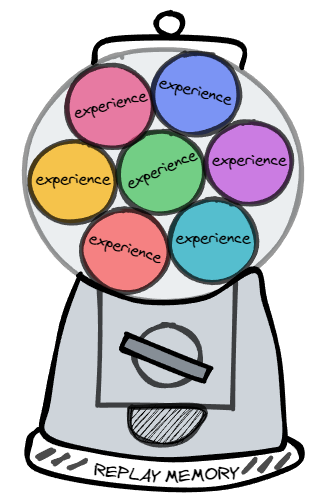
\includegraphics[scale=0.618]{pix/q_learning/replay_memory.png}
%\caption{Experience replay and replay memory}
%\label{fig:label}
\end{figure}

All of the agent's experiences at each time step over all episodes played by the agent 
are stored in the {\bf replay memory}. Well actually, in practice, we'll usually see the 
replay memory set to some finite size limit, $N$, and therefore, it will only store the 
last $N$ experiences.

This replay memory data set is what we'll randomly sample from to train the network. The 
act of gaining experience and sampling from the replay memory that stores these experience 
is called experience replay.

\subsection{Why Use Experience Replay?}

Why would we choose to train the network on random samples from replay memory, rather 
than just providing the network with the sequential experiences as they occur in the 
environment?

\begin{emp_box}
{\bf A key reason for using replay memory is to break the correlation between consecutive 
samples.}
\end{emp_box}

If the network learned only from consecutive samples of experience as they occurred 
sequentially in the environment, the samples would be highly correlated and would 
therefore lead to inefficient learning. Taking random samples from replay memory breaks 
this correlation.


\subsection{Combining A Deep $Q$-Network With Experience Replay}

Alright, we now have the idea of experience replay down. From last time, we should also 
have an understanding of a general deep $Q$-network architecture, the data that the network 
accepts, and the output from the network.

As a quick refresher, remember that the network is passed a state from the environment, 
and in turn, the network outputs the $Q$-value for each action that can be taken from 
that state.

Let's now bring all of this information in together with experience replay to see how 
they fit in with each other.


\subsubsection{Setting Up}

Before training starts, we first initialize the replay memory data set $D$ to capacity 
$N$. So, the replay memory $D$ will hold $N$ total experiences.

Next, we initialize the network with random weights. For the weight initialization in 
Deep Learning, please check out \href{https://deeplizard.com/learn/video/8krd5qKVw-Q}{weight initialization}. 

Next, for each episode, we initialize the starting state of the episode. We will talk 
about states, including the starting state, in future subsections.


\subsubsection{Gaining Experience}

Now, for each time step $t$ within the episode, we either explore the environment and 
select a random action, or we exploit the environment and select the greedy action for 
the given state that gives the highest $Q$-value. Remember, this is the exploration-
exploitation trade-off.

We then execute the selected action $a_t$ in an emulator. So, for example, if the 
selected action was to move right, then from an emulator where the actions were being 
executed in the actual game environment, the agent would actually move right. We then 
observe the reward $r_{t+1}$ given for this action, and we also observe the next state 
of the environment, $s_{t+1}$. We then store the entire experience tuple 
$e_t = (s_t, a_t, r_{t+1}, s_{t+1})$ in replay memory $D$.


\subsection{Wrapping Up on the CartPole-v0 task}

Here's a summary of what we have so far:

\begin{itemize}
%\setlength{\itemsep}{0pt}
%\setlength{\parsep}{0pt}
\setlength{\parskip}{0pt}
\item[1.]
Initialize replay memory capacity.

\item[2.]
Initialize the network with random weights.

\item[3.]
For each episode:
	\begin{itemize}
	\item[(1)]
	Initialize the starting state.

	\item[(2)]
	For each time step:
		\begin{itemize}
		\item[1)]
		Select an action.
			\begin{itemize}
			\item[-]
			Via exploration or exploitation
			\end{itemize}

		\item[2)]
		Execute selected action in an emulator.

		\item[3)]
		Observe reward and next state.

		\item[4)]
		Store experience in replay memory.
		\end{itemize}
	\end{itemize}
\end{itemize}

We’ll be using experience replay memory for training our DQN of on the CartPole-v0 task 
introduced in the last section. It stores the transitions that the agent observes, 
allowing us to reuse this data later. By sampling from it randomly, the transitions that 
build up a batch are decorrelated. It has been shown that this greatly stabilizes and 
improves the DQN training procedure.

For this, we’re going to need two classses:

\begin{itemize}
%\setlength{\itemsep}{0pt}
%\setlength{\parsep}{0pt}
\setlength{\parskip}{0pt}
\item
Transition - a named tuple representing a single transition in our environment. It 
essentially maps (state, action) pairs to their (next\_state, reward) result, with the 
state being the screen difference image as described later on.

\item
ReplayMemory - a cyclic buffer of bounded size that holds the transitions observed 
recently. It also implements a `.sample()` method for selecting a random batch of 
transitions for training.
\end{itemize}

\begin{lstlisting}[language=Python]
Transition = namedtuple('Transition',
                        ('state', 'action', 'next_state', 'reward'))


class ReplayMemory(object):

    def __init__(self, capacity):
        self.memory = deque([],maxlen=capacity)

    def push(self, *args):
        """Save a transition"""
        self.memory.append(Transition(*args))

    def sample(self, batch_size):
        return random.sample(self.memory, batch_size)

    def __len__(self):
        return len(self.memory)
\end{lstlisting}


%%%%%%%%%%%%%%%%%%%%%%%%%%%%%%%%%%%%%%%%%%%%%%%%%%%%%%%%
%
\section{Training A Deep $Q$-Network With Replay Memory}
%
%-------------------------------------------------------

% https://deeplizard.com/learn/video/0bt0SjbS3xc

In this section, we'll focus in on the complete algorithmic details of the underlying 
training process. With this, we'll see exactly how the replay memory that was introduced 
in the previous section is utilized during training as well.


\subsection{The Policy Network}

After storing an experience in replay memory, we then sample a random batch of experiences 
from replay memory. For ease of understanding, though, we're going to explain the remaining 
process for a single sample, and then you can generalize the idea to an entire batch.

Alright, so from a single experience sample from replay memory, we then preprocess the 
state (grayscale conversion, cropping, scaling, etc.), and pass the preprocessed state to 
the network as input. Going forward, we'll refer to this network as the policy network 
since its objective is to approximate the optimal policy by finding the optimal 
$Q$-function.

The input state data then forward propagates through the network, using the same forward 
propagation technique that we've discussed for any other general neural network. The model 
then outputs an estimated $Q$-value for each possible action from the given input state.

The loss is then calculated. We do this by comparing the $Q$-value output from the network 
for the action in the experience tuple we sampled and the corresponding optimal $Q$-value, 
or target $Q$-value, for the same action.

Remember, the target $Q$-value is calculated using the expression from the right hand side 
of the Bellman equation. So, just as we saw when we initially learned about plain 
$Q$-learning earlier in this chapter, the loss is calculated by subtracting the $Q$-value 
for a given state-action pair from the optimal $Q$-value for the same state-action pair.

\begin{eqnarray*}
q_{\ast }\left( s,a\right) - q(s,a) &=& loss \\
E\left[ R_{t+1}+\gamma \max_{a^{\prime }}q_{\ast }\left( s^\prime,a^{\prime }\right)\right] 
- E\left[ \sum_{k=0}^{\infty }\gamma ^{k}R_{t+k+1}\right]
&=& loss
\end{eqnarray*}


\subsection{Calculating The Max Term}

When we are calculating the optimal $Q$-value for any given state-action pair, notice 
from the equation for calculating loss that we used above, we have this term here that 
we must compute:
$$
\max_{a^{\prime }}q_{\ast }\left( s^\prime,a^{\prime }\right)
$$

Recall that $s'$ and $a'$ are the state and action that occur in the following time step. 
Previously, we were able to find this $\max$ term by peeking in the $Q$-table, remember? 
We'd just look to see which action gave us the highest $Q$-value for a given state.

Well that's old news now with deep $Q$-learning. In order to find this $\max$ term now, 
what we do is pass $s'$ to the policy network, which will output the $Q$-values for each 
state-action pair using $s'$ as the state and each of the possible next actions as $a'$. 
Given this, we can obtain the $\max$ $Q$-value over all possible actions taken from $s'$, 
giving us $\max_{a^{\prime }}q_{\ast }\left( s^\prime,a^{\prime }\right)$.

Once we find the value of this $\max$ term, we can then calculate this term for the 
original state input passed to the policy network.

\begin{eqnarray*}
E\left[ R_{t+1}+\gamma \max_{a^{\prime }}q_{\ast }\left( s^\prime,a^{\prime }\right)\right]
\end{eqnarray*}
 
Why do we need to calculate this term again?

Ah, yes, this term enables us to compute the loss between the $Q$-value given by the 
policy network for the state-action pair from our original experience tuple and the target 
optimal $Q$-value for this same state-action pair.

So, to quickly touch base, note that we first forward passed the state from our experience 
tuple to the network and got the $Q$-value for the action from our experience tuple as 
output. We then passed the next state contained in our experience tuple to the network to 
find the $\max$ Q-value among the next actions that can be taken from that state. This 
second step was done just to aid us in calculating the loss for our original state-action 
pair.

This may seem a bit odd, but let it sink in for a minute and see if the idea clicks.


\subsection{Training The Policy Network}

Alright, so after we're able to calculate the optimal $Q$-value for our state-action pair, 
we can calculate the loss from our policy network between the optimal $Q$-value and the 
$Q$-value that was output from the network for this state-action pair.

Gradient descent is then performed to update the weights in the network in attempts to 
minimize the loss, just like we've seen in all other neural networks. In this case, 
minimizing the loss means that we're aiming to make the policy network output $Q$-values 
for each state-action pair that approximate the target $Q$-values given by the Bellman 
equation.

Up to this point, everything we've gone over was all for one single time step. We then 
move on to the next time step in the episode and do this process again and again time 
after time until we reach the end of the episode. At that point, we start a new episode, 
and do that over and over again until we reach the max number of episodes we've set. We'll 
want to keep repeating this process until we've sufficiently minimized the loss.


\subsection{Wrapping Up}

Admittingly, between the last section and this one, that was quite a number of steps, so 
let's go over this summary to bring it all together.

\begin{itemize}
%\setlength{\itemsep}{0pt}
%\setlength{\parsep}{0pt}
\setlength{\parskip}{0pt}
\item[1.]
Initialize replay memory capacity.

\item[2.]
Initialize the network with random weights.

\item[3.]
For each episode:
	\begin{itemize}
	\item[(1)]
	Initialize the starting state.

	\item[(2)]
	For each time step:
		\begin{itemize}
		\item[1)]
		Select an action.
			\begin{itemize}
			\item[-]
			Via exploration or exploitation
			\end{itemize}

		\item[2)]
		Execute selected action in an emulator.

		\item[3)]
		Observe reward and next state.

		\item[4)]
		Store experience in replay memory.

		\item[5)]
		Sample random batch from replay memory.

		\item[6)]
		Preprocess states from batch.

		\item[7)]
		Pass batch of preprocessed states to policy network.

		\item[8)]
		Calculate loss between output Q-values and target Q-values.
			\begin{itemize}
			\item[-]
			Requires a second pass to the network for the next state
			\end{itemize}

		\item[9)]
		Gradient descent updates weights in the policy network to minimize loss.
		\end{itemize}
	\end{itemize}
\end{itemize}


%%%%%%%%%%%%%%%%%%%%%%%%%%%%%%%%%%%%%%%%%%%%%%%%%%%%%%%%
\section{DQN improvement}
%
% https://greentec.github.io/reinforcement-learning-third-en/
%
%-------------------------------------------------------

\subsection{Hyperparameter adjustment}

\subsection{weight initialization}

\subsection{soft update (target network)}

\subsection{Double DQN}

\subsection{Dueling DQN}




